\section{Biografie} \label{sec:bio}
In diesem Abschnitt wird das Leben von Pierre de Fermat beschrieben.

\subsection{Eltern} \label{sec:eltern}
Fermats Vater war Dominique Fermat, ein reicher Verkäufer und Hersteller. Dominique tat sein Bestes um die Familie in Reichtum aufblühen zu lassen, indem er Tauschhandel mit verschiedenen Ländern trieb. Dabei handelte er mit landwirtschaftlichen Erzeugnissen, wie z.B. Weizen, Wein, Vieh und anderen Tierprodukten. Sein Geschick und sein Ansehen haben ihn so reich werden lassen wie er geworden ist. Pierres Mutter war Claire De Long, die zweite Frau Dominiques, welche aus einer edlen Familie von Juristen kam. Durch Dominiques Ehe mit Claire De Long hatte sich die Familie außerdem die Möglichkeit bekommen, einen Platz im hohen Strafgericht von Toulouse für die beiden Söhne, Pierre und Clement, zu ergattern. Sie starb als Pierre nur sieben Jahre alt war.

\subsection{Kindheit} \label{sec:kindheit}

\begin{wrapfigure}{r}{0.25\textwidth}
    \centering
    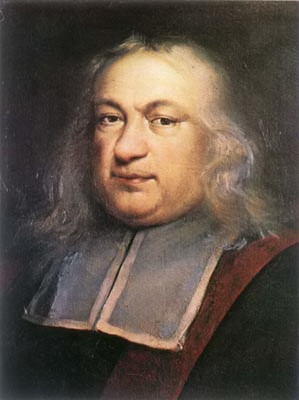
\includegraphics[width=0.25\textwidth]{Pierre_de_Fermat.jpg}
    \caption{Pierre de Fermat \cite{imgFermat}}
    \label{fig:fermat}
\end{wrapfigure}

Eines von Pierre de Fermats Rätseln ist bereits seine Geburt. In vielen Quellen wird beschrieben, dass seine Geburt 1601 in Frankreich sei. In diesem Gedanken hat man dann auch sein 400. Jubiläum im Jahr 2001 gefeiert. Seine Geburt hat sich aber schlussendlich als 1607 herausgestellt. \cite{whenWasFermatBorn} Grund für diese Verwechslung war wahrscheinlich sein verstorbener Halbbruder, welcher ebenfalls Pierre Fermat hieß, dann 1601 geboren war und noch in der Kindheit gestorben ist. \cite{famousScientistsFermat} Seine Karriere war von seinen Eltern bereits lange vorausgeplant, es ging ausschließlich darum sich einen Platz als parlamentarischen Berater, einem sogenannten \textit{\say{Conseiller}}, in Toulouse oder Bordeaux zu erkaufen. Dafür muss man mehrere Jahre Jura studiert, einen Abschluss darin gemacht, dann noch mehrere Jahre als Anwalt, entweder in Toulouse oder Bordeaux, verbracht haben und zum Schluss eine Menge Geld aufbringen um den Platz zu erwerben. Er hat den Großteil seiner Kindheit an einer sprachenzentrierten Schule verbracht, welche er im Alter von 16 Jahren abgeschlossen hatte. Dabei hat er wichtige Sprachen wie Griechisch, Latein, Italienisch und weitere gelernt und konnte diese auch flüssig sprechen, welche ihm in der späteren Laufzeit als Anwalt den Weg bahnen würde.

\subsection{Studium} \label{sec:studium}
Orléans war als die Stadt bekannt, an der man am besten Zivilrecht studieren würde. Nicht nur in Frankreich, sondern in ganz Europa. Ein Abschluss von dort wurde als sehr hoch angesehen. Dort hat er dann auch an der Universität von Orléans im August 1626 seinen Abschluss gemacht, als er nur 18 Jahre alt war. Darauf folgend hat sich Fermat im Strafgericht von Bordeaux einen Platz geschaffen. Er hat in Bordeaux die vier Jahre Praxiserfahrung als Anwalt, die für die Position des \textit{Conseillers} notwendig sind, erhalten. Eigentlich war Toulouse eine ersichtlichere Wahl gewesen, aber er hatte sich für Bordeaux für den Mathematiker-Kreis entschieden, der sich dort gebildet hatte. Er hatte nämlich damals schon Interesse an der Mathematik gefunden und ist auf die Empfehlung seines Freundes nach Bordeaux gegangen.

\subsection{Aufstieg zum Conseiller} \label{sec:aufstieg}
Als sein Vater Dominique Fermat im Juni 1628 gestorben ist, bekam Pierre den Großteil des Erbes und hat damit großen Reichtum erlangt. Er bekam mit dem Erbe sechs Bauernhöfe, so wie mehrere andere Grundstücke. Danach hatte er auf eine Gelegenheit gewartet, um sich einen Platz als \textit{Conseiller} in Toulouse zu erkaufen, um dem Plan seiner Eltern nachzugehen. Diese Gelegenheit bot sich ihm, als 1630 ein Großteil der Berater einer Pest niedergefallen sind. Solch einen Platz zu erkaufen war keineswegs billig und nur mithilfe des Erbes seines Vaters möglich. Ein einfacher Bauer hatte damals 100 Livre im Jahr verdient, während man mit dem Platz als Berater leicht mehr als 45.000 Livre los wird.

Im Jahr 1631 saß er dann endlich in seinem Büro als echter \textit{Conseiller}, durfte nun das \textit{\say{de}} in seinem Namen tragen und hieß damit offiziell \say{Pierre de Fermat} und nicht nur \say{Pierre Fermat}, ein Privileg wovon er persönlich aber nie Gebrauch gemacht hat. Um diese Zeit hat er auch seine Cousine, Louise de Long, geheiratet. Sie war zum Zeitpunkt der Hochzeit nur 15 Jahre alt. Insgesamt hatte er acht Kinder mit ihr, von denen nur fünf erwachsen geworden sind. 1637 stieg er zu einer höheren Position im Toulouser Strafgericht auf, diese Position hat er dann bis zu seinem Lebensende 1665 behalten. Mehr zu seiner Karriere als \textit{Conseiller} lässt sich in der Dezember 2001 Ausgabe der European Mathematical Society (EMS) finden. \cite{barnerNewspaper}

\subsection{Mathematik} \label{sec:biografieMathematik}
Wie für viele andere Mathematiker in der Zeit war die Mathematik für ihn nur eine Nebenbeschäftigung, da es den Beruf \say{Mathematiker} an sich noch nicht wirklich gab. Er hat zwar während seines Jura-Studiums in Orléans bereits Interesse an der Mathematik gefunden und sie auch aktiv verfolgt, aber weiterhin seinen Fokus auf das Anwaltsleben gelegt. Nach seinem Aufstieg als Berater hat er begonnen mit verschiedenen älteren Werken zu arbeiten, indem er sie restaurierte bzw. rekonstruierte. Oft hatte er mit anderen Mathematikern über einen Briefaustausch Kontakt, darunter René Descartes, Blaise Pascal und weitere. Auch wenn er nur ein Hobbyist war und als Amateur bezeichnet wird, wird er als der größte Amateur-Mathematiker aller Zeiten angesehen. \cite{mlodinow2011wenn, britannicaFermat} Wie genau er zur Mathematik beigetragen hat, wird in Kapitel \ref{sec:mathematik} behandelt.

\subsection{Als Person}\label{sec:person}
Er hat viele wichtige Dinge entdeckt, aber hatte selten das Verlangen diese zu veröffentlichen. Sein Sohn, Clement Samuel de Fermat, hatte nach Pierres Tod einige seiner Briefe und Randnotizen veröffentlicht. Sein Charakter findet sich auch in eben diesen Notizen wieder.

Im Briefaustausch mit anderen Mathematikern wurden sie oft von ihm aufgefordert ein bestimmtes Problem zu lösen, meist eines zu welchem er bereits eine Lösung hatte. Er bat sie also nicht einfach um Hilfe, sondern wollte nur schauen, wie schnell sie das Problem lösen konnten. Oder er hat eine Aufgabe mit dem Resultat, aber ohne den Lösungsweg präsentiert, falls er denn doch mal etwas veröffentlicht hatte. Seinen Charakter könnte man gut als leicht arrogant bezeichnen.

Auch hat er immer behauptet eine bestimmte Behauptung bewiesen zu haben,schrieb aber nie den Beweis dafür auf. Darunter gehören zum Beispiel auch der Zwei-Quadrate-Satz und Fermats großer Satz, welche beide in Kapitel \ref{sec:zahlentheorie} behandelt werden. Am bekanntesten wird wohl für immer folgende Behauptung bleiben, welcher als Kommentar am Buchrand in seiner Kopie von \textit{\say{Arithmetica}} von Diophantus verfasst war. Dieser würde dann zu seiner berühmtesten Problemstellung werden, welche in Kapitel \ref{sec:grSatz} näher behandelt wird.

\begin{quote}
    \say{\textit{Ich habe einen wahrlich wunderbaren Beweis für dieses Problem entdeckt, für den dieser Buchrand zu eng ist.}}
\end{quote}
